\section{JACK's User Interface}\label{SecUI}

One of the features that distinguish JACK from other program
verification tools is the integration in the IDE Eclipse. This ensures
a seamless integration of formal methods in the application
development process: the application developer does not have to learn
the peculiarities of a new tool, and does not have to switch tools to
apply formal verification techniques.

The integration in Eclipse consists of two parts: an extension of the
standard Java perspective with special JACK-related actions (checking a
specification, calling an automatic prover \emph{etc.}), and a
special JACK perspective to inspect the generated proof
obligations.

\subsection{Extension of the Java Perspective in Eclipse}

The standard Java perspective of Eclipse is extended with several
JACK-specific features. Menus are added to set the defaults for the
different specification constructs. Further, there are buttons and
menu-options to ``compile'' a JML specification, (\emph{i.e.}\ type
check and generate proof obligations), call an automatic prover on all
the generated proof obligations (either Simplify or a special
Coq tactic), or change to the special JACK perspective.  

Checking the JML specification is not done automatically, while
editing the file (as is done for Java); instead the user has to launch
this action explicitly. At the time this interface was developed,
adding such automatic checks required too many changes to the
internals of Eclipse, which were not default available. However, in
the mean time such a feature has been developed within the JMLEclipse
project\footnote{See
\texttt{http://jmleclipse.projects.cis.ksu.edu/}.}. This project also
provides syntax highlighting of JML specifications in Eclipse's Java
perspective. All this could be integrated with the JACK interface. 

%It is future work to integrate this with the JACK interface.
%%(\emph{e.g.}\ the JMLEclipse project does not accept the keywords that
%JACK adds to JML. 

Finally, another important constraint is the interface's
responsiveness. An IDE is supposed to be used interactively, and the
developer should never have to wait long for a result. Proof
obligation generation is no problem for this, but calling an automatic
prover on the generated proof obligations can take a significant
amount of time. Therefore, the prover is called in a non-blocking way,
launching a special window that allows to see the progress of the
task.

\subsection{A Proof Obligation Inspection Perspective}

An important feature of JACK is that one can inspect the different
generated proof obligations. Moreover, one does not have to understand
the specific specification language of the prover that is being used;
instead the proof obligations can be viewed in a Java/JML-like syntax
(but of course, one can also choose to see the proof obligations as
they are generated for a specific theorem prover).

\begin{figure}[t!]
%julien: at my desk it makes things bugs....
% \epsfig{file=screen1.ps,angle=270,width=\textwidth}
% the following work better (for me, with the makefile)
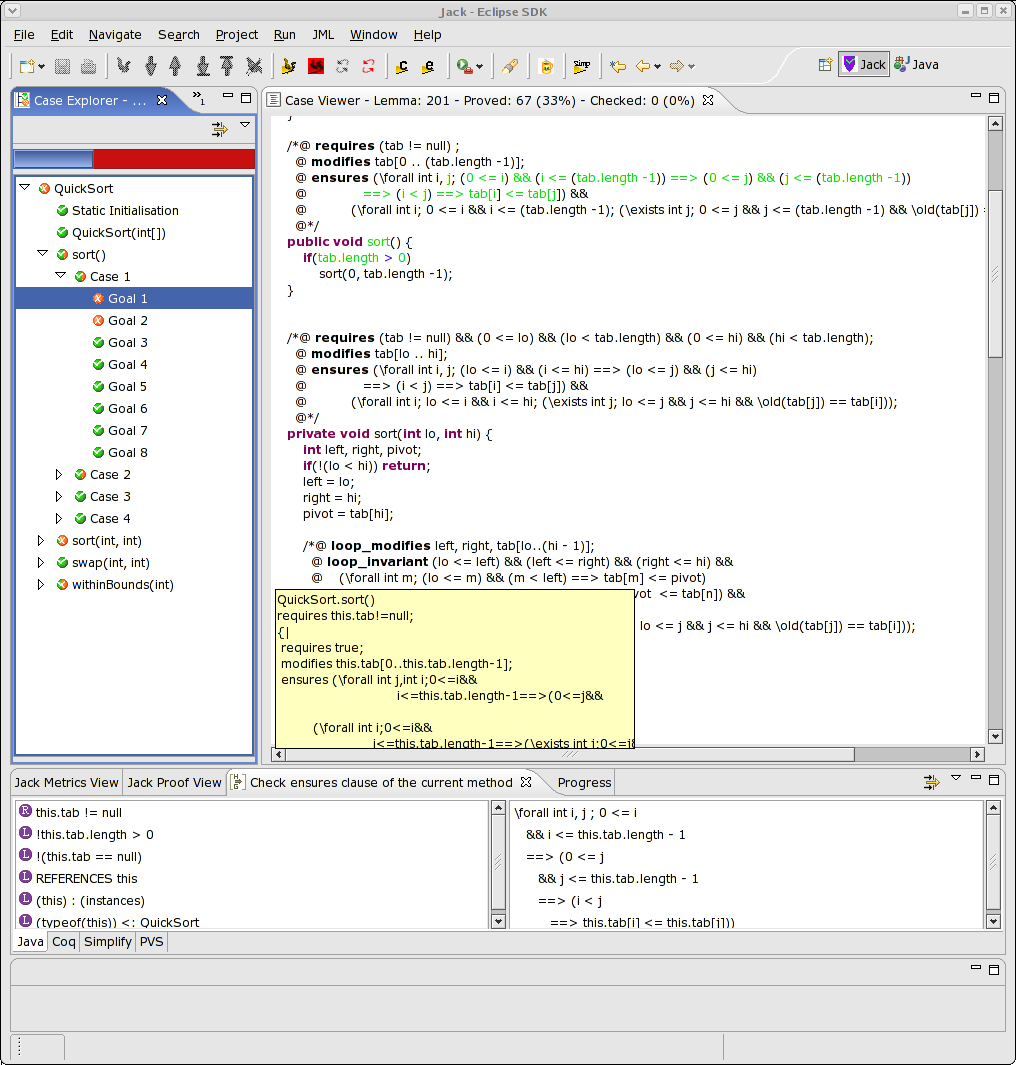
\epsfig{file=screen1, width=\textwidth}
\caption{JACK's proof obligation inspection perspective}\label{FigJackPerspective}
\end{figure}

%\begin{figure}[th!]
%    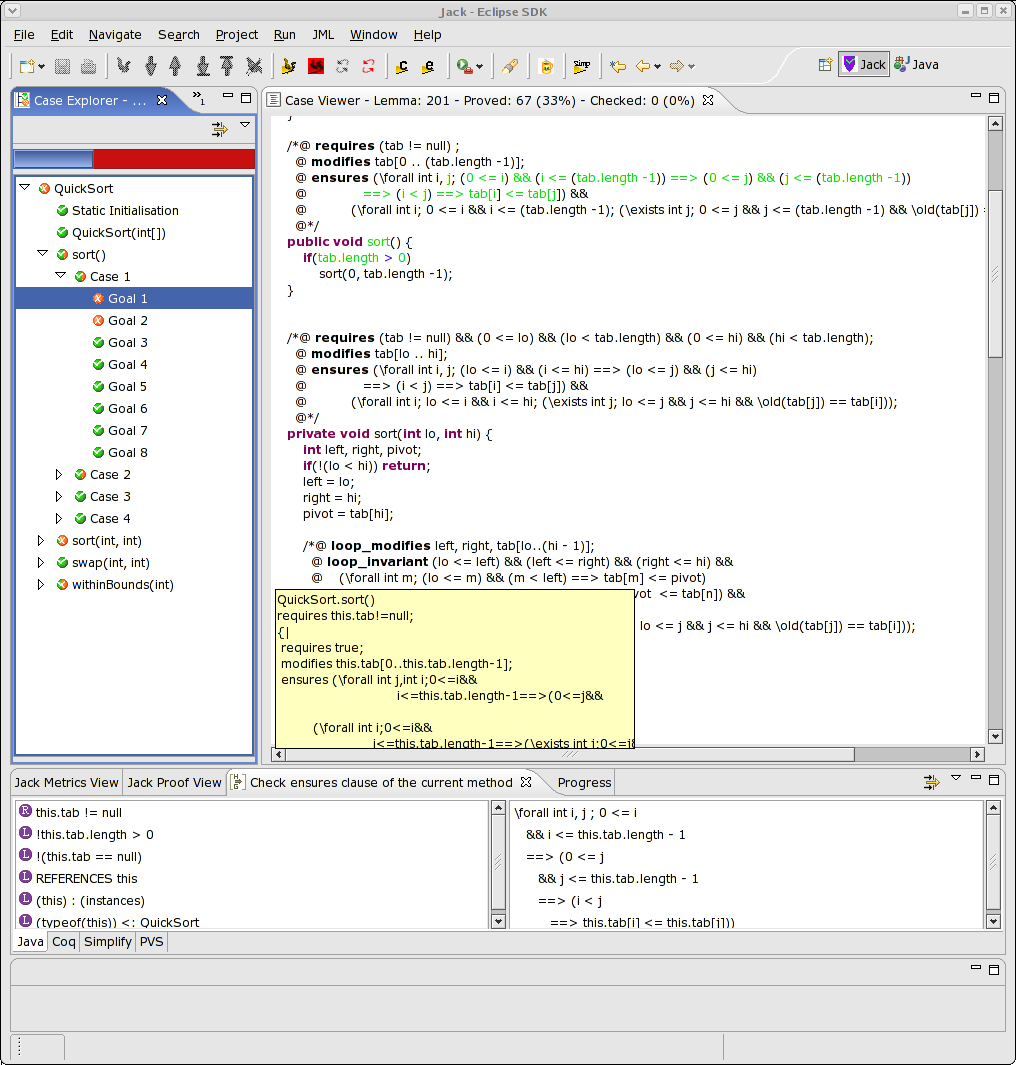
\includegraphics[width=\textwidth]{screen1}
%\caption{JACK's proof obligation inspection perspective}\label{FigJackPerspective}
%\end{figure}
%JACK's proof obligation inspection perspective provides the following information:
%\begin{itemize}
%\item information concerning the current proof status;
%\item the class methods with their lemmas;
%\item the source code; and
%\item the currently selected proof obligation (goal and hypotheses).
%\end{itemize}

Figure~\ref{FigJackPerspective} shows the inspection of a proof obligation
for the method \texttt{sort} in the QuickSort example of
Figure~\ref{FigJMLSpec}. The left upper windows allows one to browse
the proof obligations for the current class. Proven obligations are
ticked, the others are marked with a cross. The right window shows the
original source code, where the path through the code that corresponds
to the current proof obligation is coloured, together with the
relevant part of the method specification. Different colours are used
to indicate different cases, \emph{i.e.}\ to distinguish normal from
exceptional execution, and to mark that extra information is
available, such as a method specification, or the result of a
conditional expression.  The bottom window shows the proof obligation:
the left half contains the hypotheses, marked with letters indicating
their origin, \emph{e.g.}\ a hypothesis marked R originates from the
method's requires clause, while a hypothesis marked L is derived from
local declarations within the method. The right half of the window
shows the actual goal that has to be proven. The window name
highlights once again that this proof obligation originates from the
postcondition. Finally, notice that the proof obligation is here
displayed in Java syntax, but that buttons are available to change to
Coq, Simplify or PVS syntax.

%\marginpar{MH: Say something about 'manual check' option for proof
%obligations}

The user can use the proof obligation inspection view to inspect the
different (unproven) proof obligations, and to launch different
(interactive or specialised) provers to prove the remaining proof
obligations.

